\documentclass{report}

\usepackage{titletoc}
\usepackage{parskip}
\usepackage{graphicx}
\usepackage{verbatim}

\graphicspath{ {/home/anna/workspace/EquivalencesApp/report/i/} }

\makeatletter
\def\@makechapterhead#1{%
  \vspace*{50\p@}%
  {\parindent \z@ \raggedright \normalfont
    \interlinepenalty\@M
    \Huge \bfseries #1\par\nobreak
    \vskip 40\p@
  }}
  \makeatother

\begin{document} 

\title{Equivalence Teaching Tool} 
\author{Anna Thomas} 

\maketitle 

\tableofcontents 

\chapter{Introduction} 

%What is the problem, why is it interesting and what’s your main idea for solving it?

We have been challenged with developing an android application to help new students learn propositional logic and to complete logical equivalences. In this section we will discuss our motivation, approach and objectives.

\section{Motivation} 

All logics are based on propositional logic in some form, so it is important that new students learn how to use it. Propositional logic consists of syntax, semantics and proof theory; syntax is the formal language which is used to express concepts, semantics provide meaning for the language and proof theory provides a way to convert one formula into another using a defined set of rules.

We know that new students learning propositional logic can struggle to understand the rules and how they should be applied to formulae. To help with this our idea is to create an equivalence teaching tool; this will be a tablet application which will allow a user to apply rules to a formula until they have reached the desired equivalence.

\section{Approach}

We decided early on in the project that the tool should be an Android tablet application as opposed to a web or mobile one; this allows for an intuitive, interactive design while still having a large screen space.

The tool can be divided up into its main component parts: the parser, tree constructor, tree processing and tablet interface. The parser will be generated by the ANTLR4 parser generator, the tree constructor, processing code and the tablet interface will be written in Java with the interface using the Android SDK.

The parser requires a grammar to generate the relevant parser components. This will be used to parse the initial equivalence and return the ANTLR4 tree representation of the string.

The tree constructor is required to take the ANTLR4 representation of a tree and convert it into a more useful data structure which can be modified and displayed easily. The operators and atoms of the formula will be represented as nodes and leaves respectively.

Tree processing will be used to internally calculate which rules are applicable to each node and will allow us to subsequently manipulate the tree by applying these rules.

The interface will have an intuitive design displaying the current formula's formation tree (generated by the tree constructor) and allowing a user to click on the operators to apply a rule.

\section{Objectives}

The application should have some key features. These are outlined below:

\begin{enumerate}
\item Graphical tree representation of formulae

Representing the formula as a tree structure allows a user to see exactly how the formula should be read and can help them understand the order of operations. It also allows the user to click on an operator to select a rule for it; this is much more intuitive than just clicking on the whole formula and not knowing which section the rule would be applied to.

\item Undo/Redo functionality

Previous equivalent formulae will be displayed above the current formula. When an old formula is selected it will expand into tree form and the formulae below it are faded out \textit{(Undo)}. This will allow a user to perform rules on the old tree or select one of the later faded trees \textit{(Redo)}. When a rule is applied, the faded formulae will be removed from the history allowing the user to continue on from that point (Figure \ref{undo}).

\begin{figure}[ht]
    \centering
    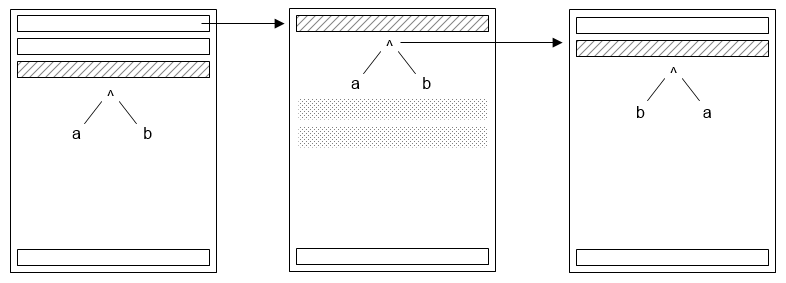
\includegraphics[width=\textwidth]{undo.png}
    \caption{Undo functionality - Clicking a previous equivalence shows the formula tree for that equivalence and sets the undone history as translucent. Applying a rule then overwrites the undone history.}
    \label{undo}
\end{figure}

\item Generated equivalences

We want to allow the user to have equivalences automatically generated for them to solve. This would be implemented by running the tool on a generated formula to give a significantly different equivalent one. The key advantage of having this feature as well as allowing manual entry of equivalences would be that the user will have a continuous supply of new equivalent logic formulae after completing all those set by their lecturer. This also requires generating the initial formula for the tool to be run upon or allowing the user to manually enter the first formula and have the second one generated for them.

\item Difficulty setting

Extending the idea of generated equivalences, we could allow the user to select a difficulty. This would be calculated by the length of the generated formula and how many rules were applied to get its equivalent formula. We could also provide a recommended difficulty based on how many previous equivalences they have completed and how far from optimal their solutions were.

\item Help

Providing the user with help is key to their improvement. Once an equivalence has been set up, the tool should calculate the optimal route from the starting formula to the desired end point. Upon finishing the equivalence the user will receive a message telling them how far from the optimal solution they were and give them the option to try again or to view the optimal solution. Throughout there will also be a help button available that will suggest the next step to the user on request; this includes the recommendation to undo certain steps if the user reaches a cycle. Pointing out mistakes could also be enabled, so if the user has completed a cycle or is heading towards a dead end they will be prompted to consider a different strategy.

\end{enumerate}


\chapter{Background}

We are assuming a basic understanding of propositional logic, including the operators and rules that are defined in the system. For more information on these please visit the Wikipedia article\cite{propositionalwiki}.

\section{Propositional Logic}

Propositional logic is a branch of logic that studies ways of combining and modifying whole sentences, statements or propositions to form more complex propositions. It is a formal system containing logical relations and properties which are derived from these methods of joining or altering statements.

A logical system contains three major parts:

\begin{enumerate}
\item Syntax - the formal language that is used to express concepts.
\item Semantics - provide meaning for the language.
\item Proof theory - provides a way to convert one formula into another using a defined set of rules.
\end{enumerate}

Logical definitions:

\begin{itemize}
\item \emph{Atomic} - A formula whose logical form is $\top$, $\bot$ or \textit{p} for an atom \textit{p}.
\item \emph{Negated atomic} - A formula of the form $\neg$\textit{p}.
\item \emph{Negated formula} - A formula of the form $\neg$\textit{A} for a formula \textit{A}.
\item \emph{Conjunction} - A formula of the form \textit{A}$\land$\textit{B}.
\item \emph{Disjunction} - A formula of the form \textit{A}$\lor$\textit{B}.
\item \emph{Implication} - A formula of the form \textit{A}$\to$\textit{B}, where \textit{A} is the \emph{antecedent} and \textit{B} is the \emph{consequent}.
\item \emph{Literal} - A formula that is either atomic or negated atomic.
\item \emph{Clause} - A disjunction of one or more literals.
\end{itemize}

A \textit{statement} is defined as a meaningful declarative sentence that is either true or false. For example, a statement could be: 

\begin{itemize}
\item `Socrates is a man.'
\item `All men live on Earth.'
\end{itemize}
A statement can be constructed of multiple parts, for example, the above statements can be combined into:

\begin{itemize}
\item `Socrates is a man and all men live on Earth.'
\end{itemize}
Each part of this statement can be considered a proposition. Propositional logic involves studying the connectives that join these such as \textit{`and'} and \textit{`or'} (to form conjunctions and disjunctions), the rules that determine the truth values of the propositions and what that means for the validity of the statement.

\section{Truth tables}

It is necessary to understand the meanings of the symbols used in a language. Truth tables are mathematical tables used in logic to compute the functional values of logical expressions. They can be used to determine whether or not a propositional logic statement is logically valid.

A \textit{situation} determines whether each propositional atom is true or false. A truth table shows all the situations the input variables can be in. We write 1 for true and 0 for false as shown below:

\vspace{5 mm}
\begin{center}
  \begin{tabular}{ || c | c || c | c || }
    \hline
    A & B & A$\land$B & A$\lor$B \\ \hline
    1 & 1 & 1 & 1 \\
    1 & 0 & 0 & 1\\
    0 & 1 & 0 & 1 \\
    0 & 0 & 0 & 0 \\
    \hline
  \end{tabular}
\end{center}
\vspace{5 mm}

Truth tables can be used to define any operators, including any new ones which might be desired.

\chapter{Android}

\section{Android vs Web app}
\subsection{Intuitive to use}
\subsection{Learning experience}
\subsection{None currently available for Android}

\section{Tablet vs Phone app}
\subsection{Screensize}
\subsection{Formation Tree would not feasible on phone app}

\section{Features}

\subsection{Multi-Touch Gestures}


Android is an operating system based on the Linux kernel which was designed primarily for touchscreen mobile devices such as smartphones and tablet computers\cite{androidwiki}.

The user interface is based around direct manipulation. This means using touch inputs that loosely correspond to real-world actions, for example swiping, tapping and pinching to control items on screen. The response to user actions is designed to be immediate and provides a fluid touch interface. It often provides haptic feedback (forces, vibrations or motions) to the user using the vibration capabilities.

Android takes advantage of internal hardware such as accelerometers, gyroscopes and proximity sensors in some applications to respond to other user actions, such as re-orientating the screen from portrait to landscape.

\section{Market Share}

Android's main competitor in the mobile platform market is Apple's iOS. In research conducted in the fourth quarter of 2012, Kantar Worldpanel Comtech showed sales of all Android smartphones worldwide outpacing the iPhone by a huge margin: 70 percent to 21 percent of the smartphone market\cite{androidstats}.

In the tablet market the iPad dominated Android's $7\verb+"+$ tablets with 53.8 percent to 42.7, which is lower than Android's smartphone market but steadily increasing.

\chapter{Related Work}

\section{Logic Daemon}

Created in Texas A\&M University, the Logic Daemon\cite{logicdaemon} is an online logic proof checker. It comprises a simple web page with two small text input boxes for the premises and conclusion and then one large text box for applying primitive rules (Figure: \ref{logicdaemon}).

While this tool does allow us to apply rules to prove equivalences we do not find it very intuitive to use at all. The interface itself looks quite unclear and isn't user friendly so it would not be suited to new students. Applying the rules to the premises is also quite confusing as it shows all the rules and does not alert the user to the fact they cannot be applied until they have already clicked on it. We found this a frustrating way of attempting a proof; as such, we intend to only display the rules that can be applied in the current situation.

However, it is a useful tool for those more knowledgeable about logic for checking proofs once they have got to grips with the interface. It also has a \textit{`Get Help'} button to suggest which rule to use next. We hope to use the idea of a help button in our project but to build upon it in order to provide more extensive help such as showing when an action has been repeated (i.e. a cycle has been reached).

We hope that our tool will be more intuitive to use because we will display formulae as formation trees with interactive nodes to apply rules with. This should provide a more straight forward way of presenting the rules to new students.

The website also provides a simple equivalence checker, well-formed formula checker and countermodel checker. These are all similar tools useful in logic but again the interface is not particularly intuitive or user friendly.

The Logic Daemon tool also provides support for first order logic which we are not planning on covering in our main tool. However, this could be implemented as an extension at the end of our project.

\begin{figure}[ht]
    \centering
    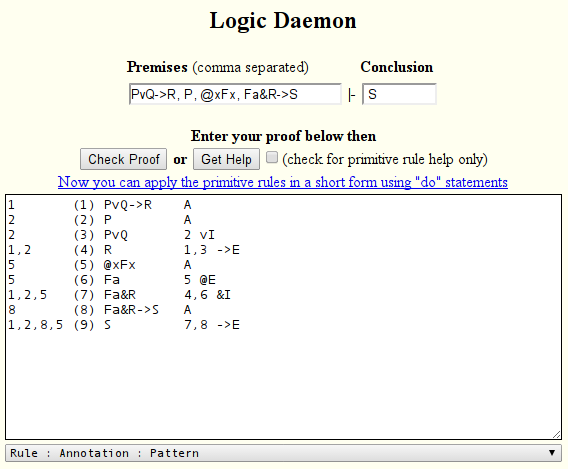
\includegraphics[width=\textwidth]{logicdaemon.png}
    \caption{Logic Daemon}
    \label{logicdaemon}
\end{figure}

\section{Pandora}

Pandora\cite{pandora} is a tool created by Imperial College London; it stands for `Proof Assistant for Natural Deduction using Organised Rectangular Areas'. It can be used to prove that a goal formula follows from the given formulae. Pandora allows the user to repeatedly apply natural deduction rules (Figure: \ref{pandora}).

We do not intend to include natural deduction in our tool as we want to focus more on solving propositional logic equivalences. Pandora is a much nicer tool than the Logic Daemon and we find it much more intuitive and easy to use.

Pandora allows a user to apply rules forwards or backwards. We know from using Pandora that some proofs are easier to complete working backwards; as such, this is an idea we hope to incorporate into our tool by allowing the user to expand either the top or bottom formula to show its formation tree and to apply rules. 

\begin{figure}[ht]
    \centering
    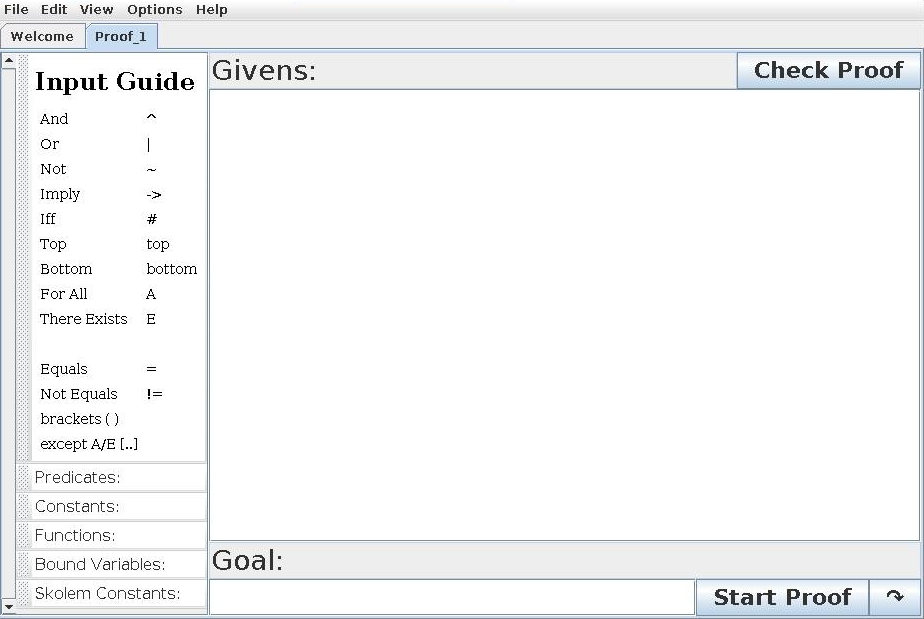
\includegraphics[width=\textwidth]{pandora.jpg}
    \caption{Pandora}
    \label{pandora}
\end{figure}

\section{Logic Solver}

This is an Android application to show truth tables and possible logical equivalences. It looks like it has been made as a phone application as on a tablet it fills very little of the screen and it is difficult to click on some of the links (Figure \ref{logicsolver}).

The user can apply rules to the formula they enter into the application; this is done by selecting the rule they want out of a list which is then applied to the formula. However they cannot use this application to solve an equivalence as they can only enter one formula and then apply rules to that. We want to improve upon this in our own application by allowing the user to enter two formulae and work from either end to solve it.

The list of rules that is offered to the user only shows the rules that can be applied to the current formula. We want to also offer this behaviour as there are far too many rules to display them all to the user and expect them to sort through which could be applied.

Formulae are displayed simply in the application; we think this could be improved upon and want to display our current formula as its formation tree.

\begin{figure}[ht]
    \centering
    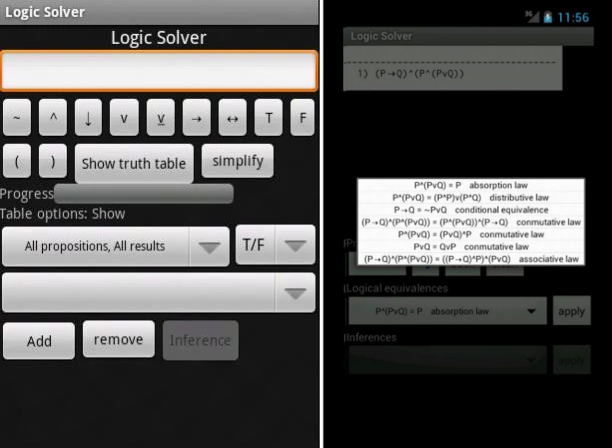
\includegraphics[width=\textwidth]{logicsolver.png}
    \caption{Logic Solver Android Application}
    \label{logicsolver}
\end{figure}

\section{Truth Tables}

Truth Tables is also an Android application mainly for use on a phone. It simply generates and displays truth tables based on a logical formula (Figure \ref{truthtables}).

We currently do not plan on adding truth tables to our application as we do not believe it is as useful for learning and understanding propositional logic as our other ideas. However, this could be added as an extension at the end of the project depending on how much time is left.

\begin{figure}[ht]
    \centering
    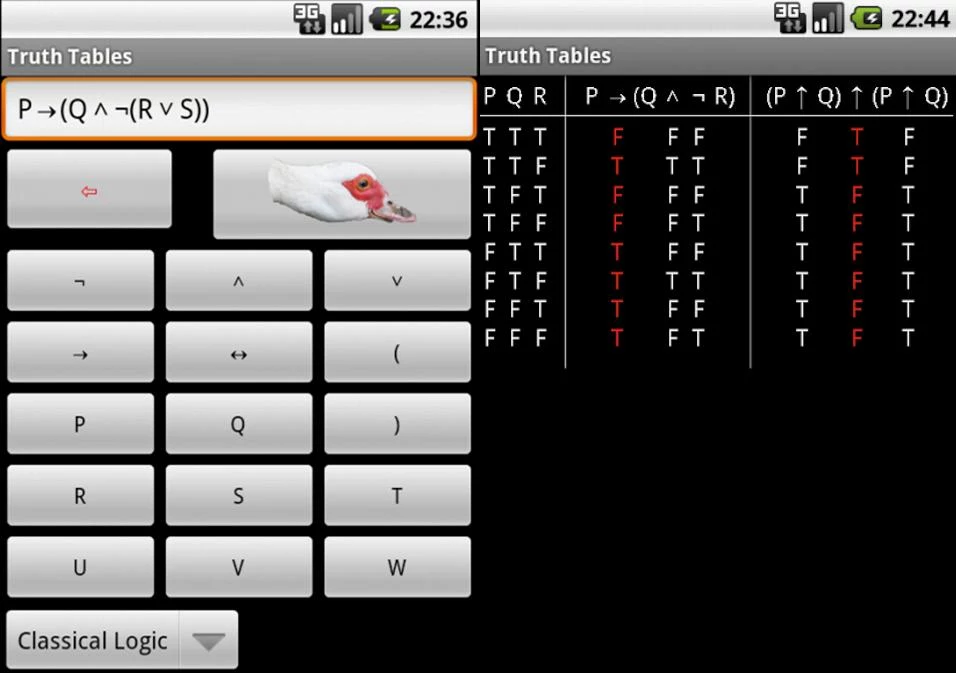
\includegraphics[width=\textwidth]{truthtables.png}
    \caption{Truth Tables Android Application}
    \label{truthtables}
\end{figure}

\section{LogicCalc}

LogicCalc is an Android application for solving problems with propositional logic. It allows the user to create workbooks to save and print their proofs (Figure \ref{logiccalcapp}). However we had trouble running it on our Nexus tablet.

We like the idea of saving proofs in workbooks for future reference. This is something we had not considered before and are curious to explore as an extension. This functionality would be useful for students completing exercises that needed a paper hand in as they would be able to save and print them off.

\begin{figure}[ht]
    \centering
    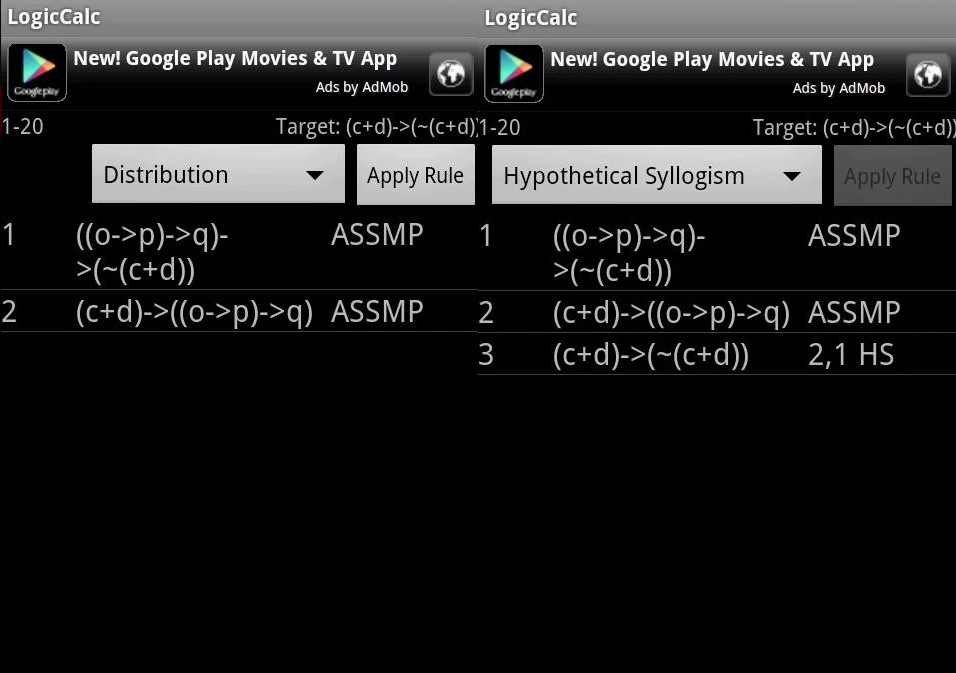
\includegraphics[width=\textwidth]{logiccalcapp.png}
    \caption{LogicCalc Android Application}
    \label{logiccalcapp}
\end{figure}

\section{Propositional Logic Calculator}

The Propositional Logic Calculator\cite{logiccalc} finds all of the models of a given propositional formula. The website tells us that the only limitation for this calculator is that we have only three atomic propositions to choose from: p,q and r (Figure: \ref{logiccalc}).

Propositions are entered using the keyboard they provide on the calculator and the reasoning process is initiated by clicking `ENTER'. It then calculates the truth value assignments that will make the formula true in the `MODELS' section and the truth value assignments making the formula false in the `COUNTERMODELS' section.

This tool is used simply for calculating truth values of a formula. We will not be implementing this in our equivalences tool because we do not think that knowing the truth values for a formula is as useful for learning and understanding propositional logic as our other ideas.

\begin{figure}[ht]
    \centering
    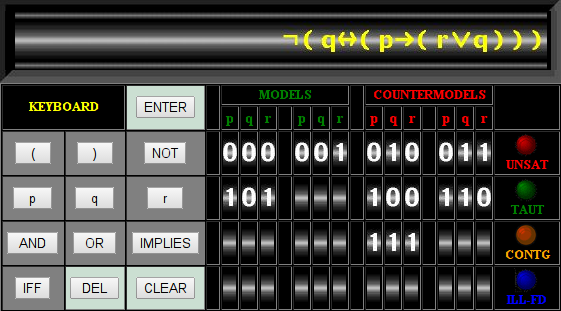
\includegraphics[width=\textwidth]{logiccalc.png}
    \caption{Propositional Logic Calculator}
    \label{logiccalc}
\end{figure}

\section{Previous Year Projects}

Once we have made more progress on our tool we will look into finding out what previous years did when they were assigned similar projects. We do not want to look into these this early in the project so we can generate our own implementation ideas as these projects will be very similar to ours.

\chapter{Parser}
\section{Parser Generation}
\subsection{ANTLR4 and alternatives}

\section{Grammar}
\subsection{Tokens}
\subsection{Order of Precedence}
\subsection{Error Handling - Incorrect grammar syntax to handle errors semantically}
\subsection{Extension to First Order Logic}

\section{Parser}
\subsection{Parser}
\subsection{Walker}

\chapter{Internal Tree Representation}
\section{Compiler}

\section{Formation Tree}
\subsection{Tree operations, eg. adding a new node}

\section{Nodes}
\subsection{Binary Operators}
\subsection{Unary Operators}
\subsection{Atoms}

\chapter{Tree Manipulation}
\section{The Rule Engine}
\section{Rule Selection - which rules can be applied to a node}
\section{Rule Application - how rules are applied to a node}
\section{Random Rule Application}
\subsection{Generating equivalent formulae}

\chapter{The App}
\section{Truth Tables}
\subsection{Ensure equivalences are equal before beginning}

\section{Random Generation of Equivalences}
\subsection{Generating single equivalence}
\subsection{Generate equivalence formula - repeated application of random rules}

\section{Custom Keyboard}
\subsection{Logic symbols and variables}

\section{Undo/Redo Functionality}
\subsection{Stack of trees maintained}
\subsection{OnClick listeners}

\section{Formation Tree Representation}
\subsection{Aims: To draw attractive tree}
\subsection{Problems: NP complete problem}
\subsection{Tree Layout}
\subsection{Walker's Algorithm}
\subsection{Alternatives}

\section{Rule Application}
\subsection{How rules are displayed within the app}

\section{Difficulty}
\subsection{Length of generated equivalences}
\subsection{Number of variables/operators}
\subsection{Number of rules different}

\section{Help}
\subsection{Detecting cycles}

\begin{comment}
\chapter{Project Plan}

\section{Progress}

\begin{enumerate}
\item Grammar and parser generator - We have created a grammar written in ANTLR4 to define the parser generator. This can take an input formula, parse it, and convert it into a tree structure that we can manipulate.
\end{enumerate}

\section{Future Plan}

Targets for March 28th (End of second term):

\begin{enumerate}
\item Tree Constructor - We need to convert the tree generated by the parser into a more useful data structure. This will be a tree where the nodes and leaves are operators and propositional atoms respectively.
\item Tree Processing - Once we have a useful data structure, we can begin manipulating it with logical rules. This will make up the internal functionality of the application. For this we will need to design some specific algorithms, for example:

\begin{itemize}
\item Rule calculator - Calculate which rules are applicable to each operator
\item Subtree manipulator - Replace subtrees based on the rule that is applied to the operator
\end{itemize}

\item Basic android interface - We will create a basic interactive interface to allow the user to enter an equivalence, display the current equivalence and apply the tree manipulation algorithms we have created. This will not display the formulae as trees yet, as we anticipate the layout will be fairly complex to design to be aesthetically pleasing.
\end{enumerate}

The goal of the rule generator is not only to generate rules to apply to the current formula but to also determine the optimal number of rules to complete the equivalence. This will be used in for generating equivalences, helping the user and spotting mistakes.

Targets for 3rd term:

\begin{enumerate}
\item Android Tree Layout - We need to design a layout algorithm (or adapt an existing one) to display the current formula as a tree so that the whole tree will be visible on the tablet as well as allowing for space for the lines of other equivalences.
\item Formula Generator - The user should be able to generate equivalences on demand to practice with as well as inputting them manually. This will function by generating an initial equation, then randomly applying a number of valid rules to the equation. This should check for cycles so that the second formula is not too similar to the first.
\item Extensions:

\begin{itemize}
\item Undo Functionality - We want the user to have the ability to undo previous rules and view the tree of a previous equivalence. When the user selects a previous equivalence they should be able to redo any steps until they decide to apply a new rule, in which case the undone history will be lost. This will be implemented by maintaining a stack for each of undo and redo.
\item Help - We want to create a help tool that uses the rule calculator to determine the optimal path from one equivalence to another. This will be used to:

\begin{itemize}
\item On request tell the user what the next optimal step is. It should generate the optimal path from their \textit{current} formula so the calculation can either be run whenever the user requests help or every step depending on how computationally expensive it is.
\item Calculate how far from the optimal path they are once they have completed the equivalence.
\item Detect if the user has made a mistake such as completing a cycle or heading towards a dead-end and prompt them.
\end{itemize}
  
\item Difficulty Settings - We want to set difficulty in a variety of ways, these include:

\begin{itemize}
\item When generating equivalences, the start formula length can be varied and rules can be applied more or fewer times depending on difficulty.
\item No help functionality for higher difficulties.
\item There is also the possibility of recommending a difficulty for the user based on how many previous equivalences they have completed, or how close their solutions have been to the optimum.
\end{itemize}

\item Extra operators - New operators could be added to the grammar such as XOR and NAND. These could be implemented as a separate grammar and they are likely to be used separately from the standard set of operators.
\end{itemize}

\end{enumerate}

\end{comment}

\chapter{Evaluation}
\section{Testing}
\subsection{JUnit tests}
\subsection{Survey - People who do/don't understand logic}

\section{Performance}

Once the application has been built we will need to find a way to test that it has met the objectives we set out to achieve. The main objective is to create an intuitive Android application that helps students improve in solving equivalences; as such, we will survey a wide range of test subjects. These tests will be split into two groups: people who understand logic and equivalences well and people who are new to propositional logic.

We need to ask people who understand logic (e.g. lecturers) so we can confirm that it works as a teaching tool. People who are new to logic (e.g. first year students) are necessary so we can evaluate how effective it is as a learning tool. This can be carried out through asking the target groups to use the application and provide feedback.

\chapter{Conclusions}
\section{Completed objectives}
\section{Comparisons to related work}

\chapter{Future Work}
\section{Improvements to completed objectives}

\section{Device support}
\subsection{Reduced app without trees for phones}

\section{More complex help}
\subsection{Calculating the optimal route}
\subsection{Suggested next move}
\subsection{Future dead end detection}

\section{First Order Logic}
\subsection{Extend grammar}
\subsection{Add and handle new rules}

\begin{thebibliography}{9}

\bibitem{propositionalwiki}
  Wikipedia,
  \emph{Propositional Logic}.
  http://en.wikipedia.org/wiki/Propositional\_calculus

\bibitem{propositionaliep}
  IEP,
  \emph{Propositional Logic}.
  http://www.iep.utm.edu/prop-log

\bibitem{androidwiki}
  Wikipedia,
  \emph{Android (Operating System)}.
  http://en.wikipedia.org/wiki/\\Android\_(operating\_system)

\bibitem{androidstats}
  Harry McCracken,
  \emph{Who’s Winning, iOS or Android?}.
  http://techland.time\\.com/2013/04/16/ios-vs-android

\bibitem{logicdaemon}
  Colin Allen, Chris Menzel,
  \emph{Logic Daemon}.
  http://logic.tamu.edu

\bibitem{pandora}
  Imperial College London,
  \emph{Pandora}.
  http://www.doc.ic.ac.uk/pandora/newpandora/\\index.html

\bibitem{logiccalc}
  Enrico Franconi,
  \emph{Propositional Logic Calculator}.
  http://www.inf.unibz.it/\\\textasciitilde franconi/teaching/propcalc

\end{thebibliography}

\chapter{User Guide}
\section{How to use the app}

\end{document}